\section{Introduction}
\label{sec:intro}


The Gauss-Bonnet theorem states that, given a surface, the sum of the curvature
at each point is equal to $2\pi$ times the Euler characteristic.
The theorem is a bridge between topological
and geometric information, see \figref{bridge}. 
This bridge can be traversed in both directions.
That is, if one has geometric information one obtains topological information and
if one has topological information one obtains geometric information.


\begin{figure}[htb]
\centering
\includegraphics[width=.3\textwidth]{curvature/bridge}
\caption{The Gauss-Bonnet theorem allowing bi-directional traffic
between geometry and topology.}
\label{fig:bridge}
\end{figure}

In the book \emph{Using the Borsuk-Ulam Theorem}
\cite{jm08},
Matou\v{s}ek states that a theorem is a great theorem if there are
\begin{enumerate}[(1)]
\item several different equivalent versions,
\item many different proofs,
\item a host of extensions and generalizations, and
\item numerous interesting applications.
\end{enumerate}

By this criteria, the Gauss-Bonnet theorem is a great theorem.
For (1), six\todo{verify} different versions of the theorem are discussed
in \cite{wu_historical_2008}. 
We highlight a version for smooth surfaces in $\RR^3$ and
 a several discrete versions for triangulated surfaces. 
 Versions exist for surface with boundary even with cusps on
 the boundary.
 Local and global versions are given in \cite{doc76}.
Versions exist for higher dimensions \cite{guillemin_differential_2010}.
The versions we discuss are extrinsic, meaning they depend on an embedding
into $\R^n$, an intrinsic version, not depending on an embedding,
 is given in \cite{chern_simple_1944}.
 
 
As for (2), often, a proof of the Gauss-Bonnet theorem appears toward
the end of introductory textbooks on differential geometry relying on the ideas
developed in the text \cite{guillemin_differential_2010,pressley_elementary_2010}.
The most common proof is to first prove the theorem for simply connected domains
with boundary, then triangulate a surface and add up the contribution from each triangle.
The disadvantage of these proofs is that they do not provide geometric intuition \cite{wu_historical_2008},
but inorder to limit the number of definition included in the background,
we give proof using this strategy.
Several fundamentally different proofs exist.
For example, in \cite{guillemin_differential_2010}, 
the Poincar\'{e}-Hopf Theorem is used,
in \cite{doc76} Green's theorem is used.
A proof based on the calculus of
moving surfaces is given in \cite{grinfeld_introduction_2013}.\todo{other versions?}
For (3), two prominent generalizations include
the Chern-Gauss-Bonnet theorem \cite{chern_simple_1944} and the Atiyah–Singer index 
theorem \cite{atiyah_index_1963}.
This work is dedicated to (4).
Most, but not all, of our applications are related to geometric algorithms. 
We did not include any of the seven applications given in \cite{doc76}.
For applications to physics see \cite{tirado-physics-apps,gibbons_applications_2008}.
A historical survey of the theorem is given in \cite{wu_historical_2008}.


\subsection{Simple Polygons}
\label{sec:warm-up}

To get a sense of the types of problems we will encounter,
we begin by deriving a formula for the area
of a simple polygon on the sphere in terms of the 
interior angles.
\begin{theorem}\label{thm:triangle}
In the plane, the sum of the interior angles of a triangle is $\pi$.
\end{theorem}
\begin{proof}
Draw a line parallel to one edge through the opposite vertex.
By alternating interior angles in the plane, the sum of the angles
in the triangle equal  a straight line.
See \figref{angles} for an illustration. 



\begin{figure}[htb]
\centering
\includegraphics[width=.3\textwidth]{background/interior-angles-triangle}
\caption{A proof that, in the plane, the sum of the angles of a triangle is $\pi$.}
\label{fig:angles}
\end{figure}

\end{proof}



Consider any simple polygon in the plane $P$ with $n$ vertices. 
Then $P$ can be triangulated with $n-2$ triangles \cite{orourke_computational_1994}.
Thus, when we traverse $P$ we go around $n-2$ triangles each contributing
$\pi$.
We have
\begin{corollary}\label{cor:angles}
In the plane, any simple polygon $P$ with $n$ vertices,
the sum of the interior angles of $P$ is $(n-2)\pi$.

\end{corollary}

Now consider a triangle on the two dimensional sphere as in \figref{sphere-triangle}.

\begin{figure}[htb]
\centering
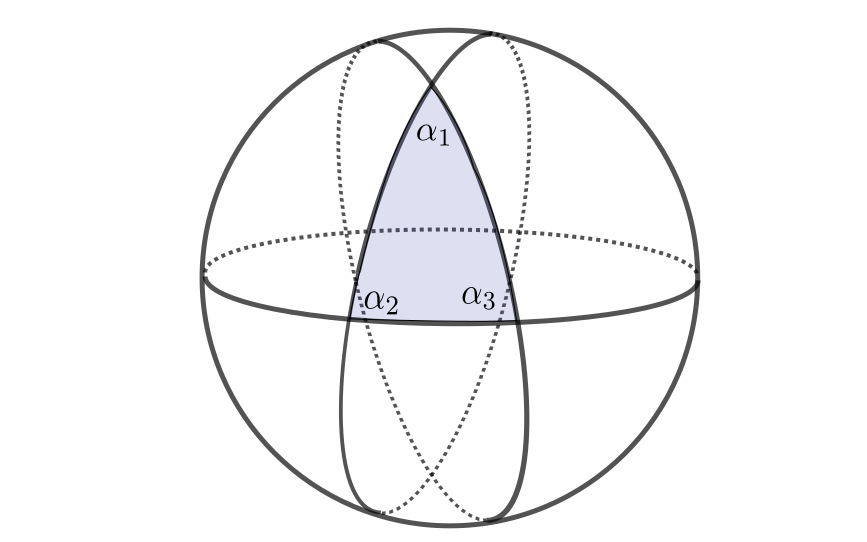
\includegraphics[width=.5\textwidth]{background/sphere-triangle}
\caption{A triangle on the sphere.}
\label{fig:sphere-triangle}
\end{figure}


\begin{figure}[htb]
\centering
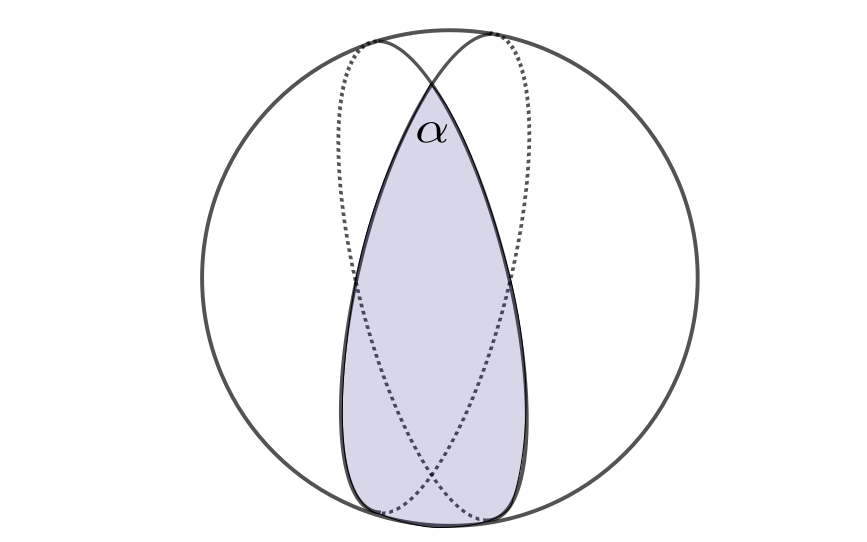
\includegraphics[width=.4\textwidth]{background/lune}
\caption{A lune with angle $\alpha$.}
\label{fig:lune}
\end{figure}

The remainder of this paper is organized as follows:
in \secref{background} we introduce definitions and notation that will be used
throughout the paper. We then state and prove the theorem.
In each subsection of \secref{applications}, we present an application of the theorem.
These subsections are independent.
I hope that the number of applications continues to grow,
please share any that you feel
ought to be included\footnote{\text{bradleymccoy@montana.edu}}.

